\begin{figure}
    \begin{center}
    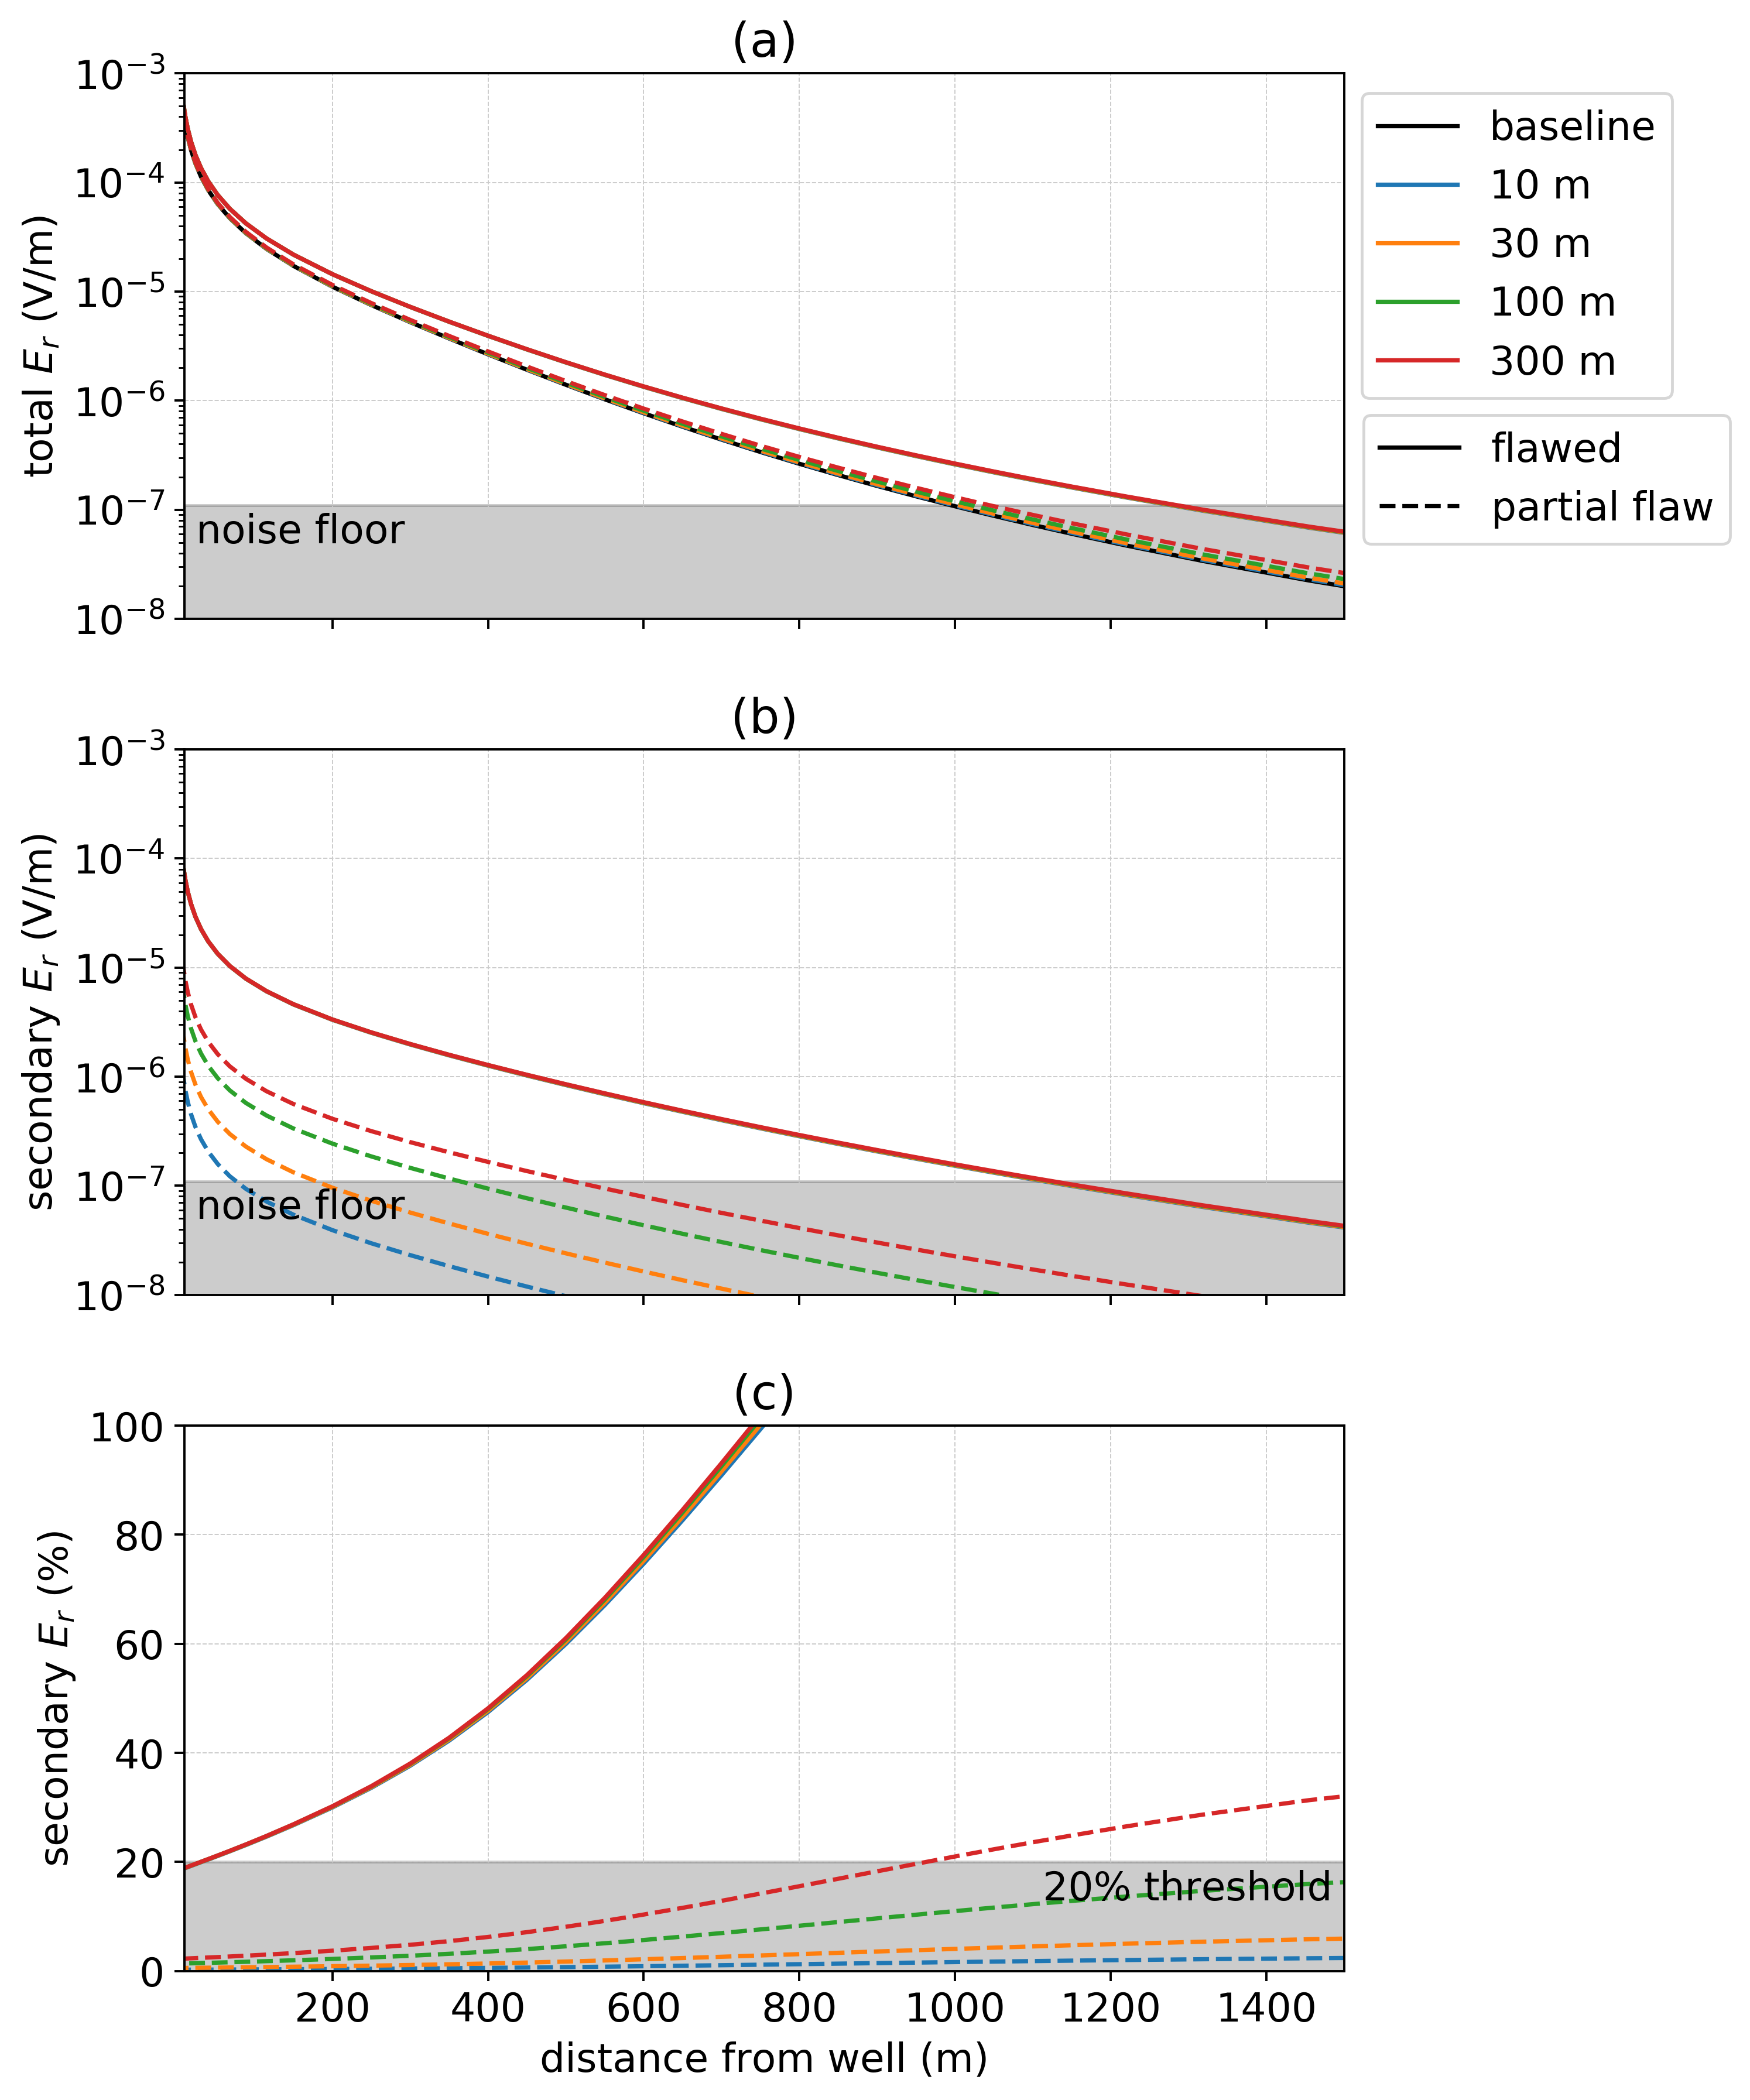
\includegraphics[width=0.8\textwidth]{figures/integrity_partial_flaw.png}
    \end{center}
\caption{
    Radial electric field as the vertical extent of the flaw is varied.
    The positive electrode is connected to the top of the casing, the negative electrode
    is positioned 500 m away and data are measured along a line $90^\circ$ from the
    source electrodes. In (a), we show the total electric field corresponding to four different flaw extents.
    The black line shows the response of the intact well.
    The dashed lines indicate the partially flawed wells (50\% of the circumference is compromised)
    and the solid lines flawed wells in which the entire circumference of the well has been compromised.
    In (b), the secondary radial electric field is plotted (with respect to an intact well primary)
    and in (c), we show the secondary radial electric field as a percentage of the primary.
}
\label{fig:integrity_partial_flaw}
\end{figure}
